\documentclass[a4paper, 12pt]{article}

%\usepackage{cmap}
\usepackage[T2A]{fontenc}
\usepackage[utf8]{inputenc}
\usepackage[english, russian]{babel}
\usepackage{graphicx}
\usepackage[top=1in, bottom=1in, left=3.2cm, right=2.6cm]{geometry}
\linespread{1.5}
\usepackage{biblatex}
\addbibresource{lib.bib}
\graphicspath{./}

\usepackage{listings}
\usepackage{color}


\begin{document}
	
\begin{titlepage}
	\fontsize{12pt}{12pt}\selectfont
	\begin{figure}[t!]
		\centering
		
\includegraphics[scale=0.8]{bmstu}
	\end{figure}
	
	\noindent\rule{15cm}{3pt}
	\newline\newline
	\noindent 
	ФАКУЛЬТЕТ 
	\underline{«Информатика и системы управления»} \newline\newline
	
	\noindent КАФЕДРА \underline{«Программное обеспечение ЭВМ и информационные технологии»}\newline\newline\newline\newline\newline\newline
	
	\centering {\LARGE Отчет по лабораторной работе № 3}
	\vspace{3mm}
	
	\centering {\LARGE По курсу "Анализ Алгоритмов"
	\vspace{10mm}	
		
	\centering \bf Трудоемкость сортировок}
	\vspace{10mm}
	
	
	\begin{flushright}
		{\large	Студент:\\ Турсунов Жасурбек Рустамович \\ Группа: ИУ7-56Б
			\vspace{5mm}
			\\Преподователи: \\ Волкова Лилия Леонидовна \\ Строганов Юрий Владимирович}
	\end{flushright}
	
	\begin{center}
		\vfill
		Москва, \the\year
		~г.
	\end{center}
\end{titlepage}

\tableofcontents
\clearpage
\newpage

\section*{Введение}

\begin{flushleft}
	\hspace*{5mm} Целью данной лабораторной работы является изучение применений алгоритмов сортировки и обучение расчету трудоемкости алгоритмов. В данной лабораторной работе рассматриваются алгоритмы сортировки пузырьком,  вставкми, а также гномья сортировка. Также требуется сделать сравнение этих алгоритмов, чтобы выбрать наилучше подходящее в конкретном случае. 
	\newline \hspace*{5mm} В ходе лабораторной предстоит выполнить следующие задачи: 
	\begin{enumerate}
		\item изучить алгоритмы сортировки;
		\item вычислить трудоемкость каждого алгоритма;
		\item реализовать три алгоритма сортировки на одном из языков программирования;
		\item сравнить алгоритмы сортировки массива.
    \end{enumerate}
		
\end{flushleft}
\clearpage
\newpage
\section{Аналитическая часть}
\begin{flushleft}
	\hspace*{5mm} Сортировкой массива - одна из самых популярных операций над массивом.\cite{sortIntro} Алгоритмы реализуют упорядочивание элементов в списке. В случае, когда элемент списка имеет несколько полей, поле, служащее критерием порядка, называется ключом сортировки.
	\newline Область применения:
	\begin{itemize}
		\item физика;
		\item математика;
		\item экономика;
		\item информатика;
		\item и тд. 
	\end{itemize}
	\subsection{Сортировка пузырьком}
	\hspace*{5mm} Алгоритм проходит по массиву n-1 раз до тех пор, пока массив не будет полностью отсортирован. В каждом проходе элементы попарно сраниваются и, при необходимости, меняются местами. При каждом проходе алгоритма по внутреннему циклу, очередной наибольший элемент ставится на своё место в конец неотсортированного массива. Таким образом наибольшие элементы "всплывают" как пузырёк.
	
	\subsection{Сортировка вставками}
	\hspace*{5mm} На каждом шаге выбирается один из элементов неотсортированной части массива (максимальный/минимальный) и помещается на нужную позицию в отсортированную часть массива.
	
	\subsection{Гномья сортировка}
	\hspace*{5mm} В данном алгоритме поддерживается указатель на текущий элемент, если он больше предыдущего или он первый — указатель смещается на позицию вправо, иначе текущий и предыдущий элементы меняются местами и  указатель сместится влево. Алгоритм похож на сортировку вставками. Главное отличие от сортировки вставками заключается в том, что перед вставкой на нужное место происходит серия обменов, как в сортировке пузырьком.
\end{flushleft}

\newpage
\section{Конструкторская часть}
\begin{flushleft}
	{\bf Требования к вводу: } На вход подается массив.
	{\bf Требования к программе: } На вход подается массив.
	\begin{enumerate}
		\item корректная сортировка массива;
		\item при нулевой длине массива программа не должнв аварийно завершаться. 
	\end{enumerate}

	\subsection{Разработка алгоритмов}
	В данном разделе будут рассмотрены схемы алгоритмов:
	\begin{enumerate}
		\item сортировка пузырьком;
		\item сортировка вставками;
		\item гномья сортировка.
	\end{enumerate}
	\clearpage
	\newpage
	\hspace*{5mm} На рисунке 1 представлена схема алгоритма сортировки пузырьком.
	\begin{figure}[h!]
		\centering 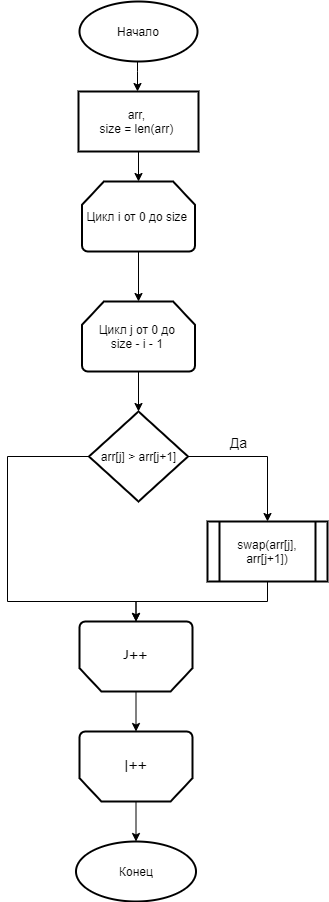
\includegraphics[scale=2.2]{bubble_graph}
		\centering \caption{Схема алгоритма сортировки пузырьком}
	\end{figure}
	\clearpage
	\newpage
	\hspace*{5mm} На рисунке 2 представлена схема алгоритма сортировки вставками.
	\begin{figure}[h]
		\centering 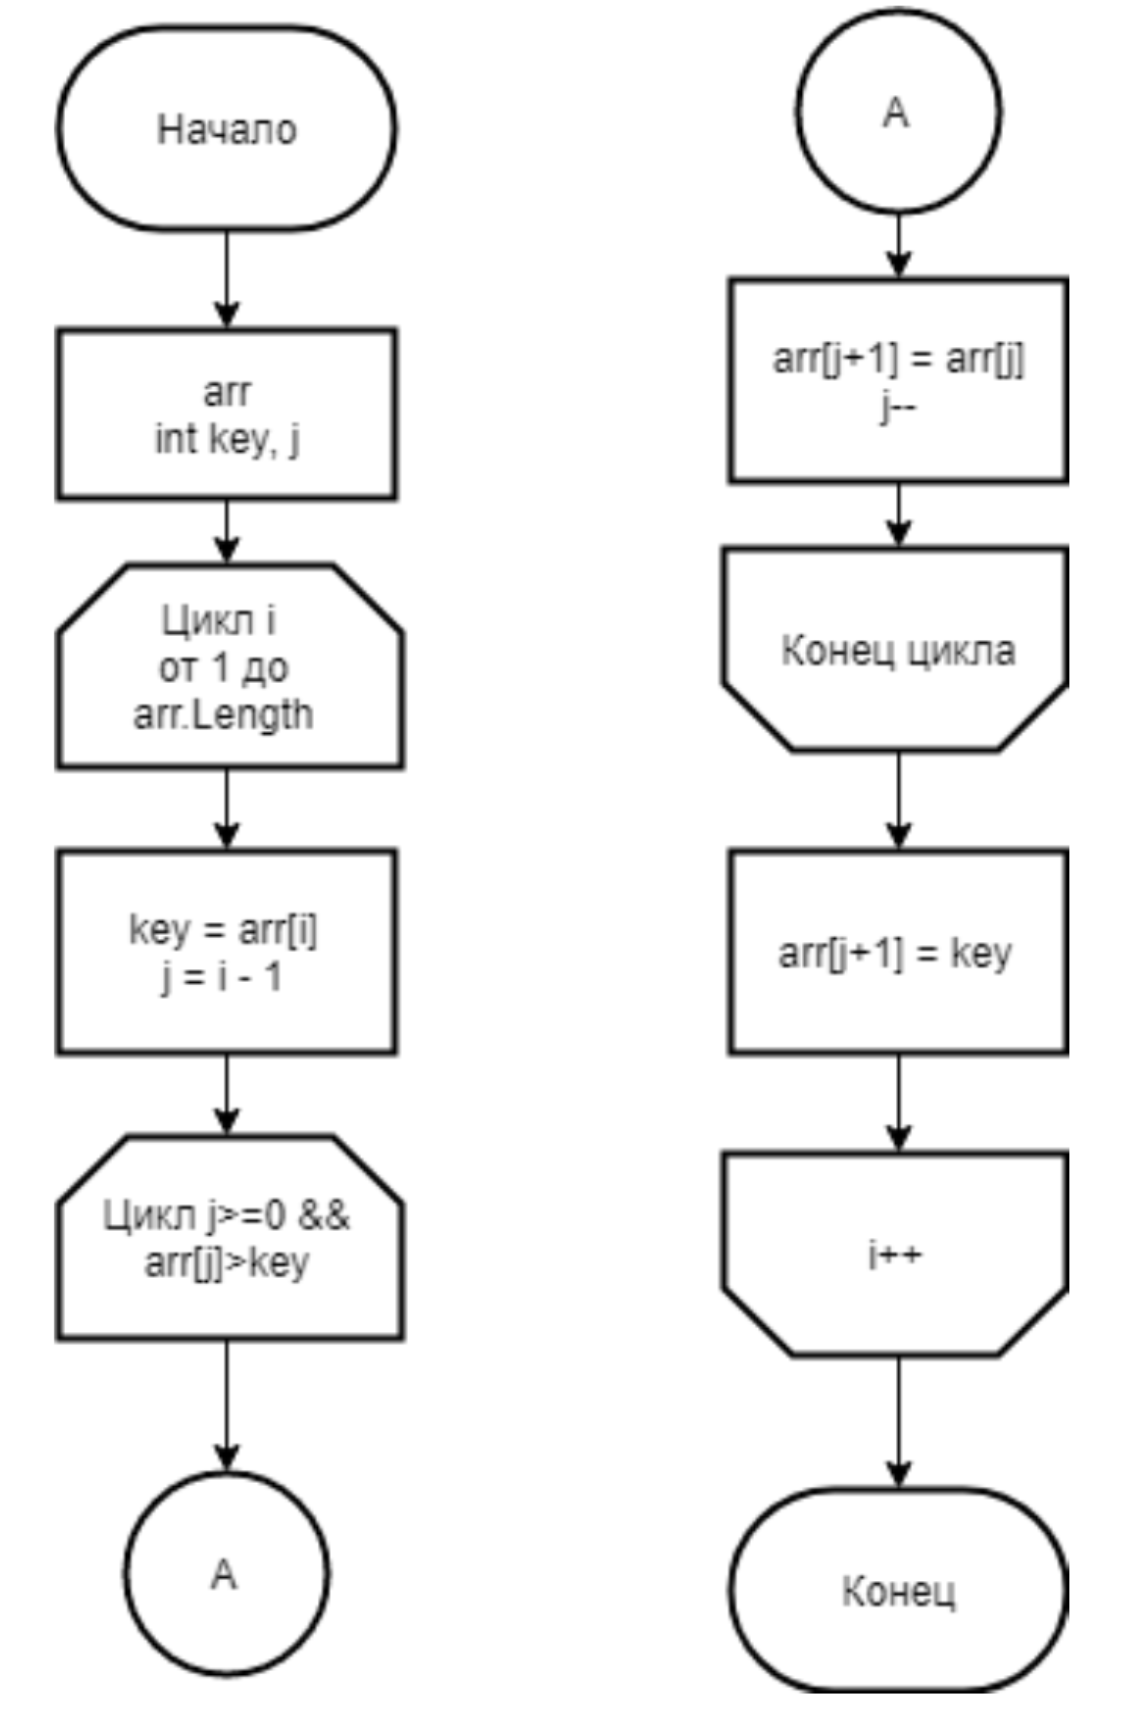
\includegraphics[scale=0.9]{insert_graph}
		\centering \caption{Схема алгоритма сортировки вставками}
	\end{figure}
    \clearpage
	\newpage
	\hspace*{5mm} На рисунке 3 представлена схема алгоритма гномьи сортировки.
	\begin{figure}[h!]
		\centering 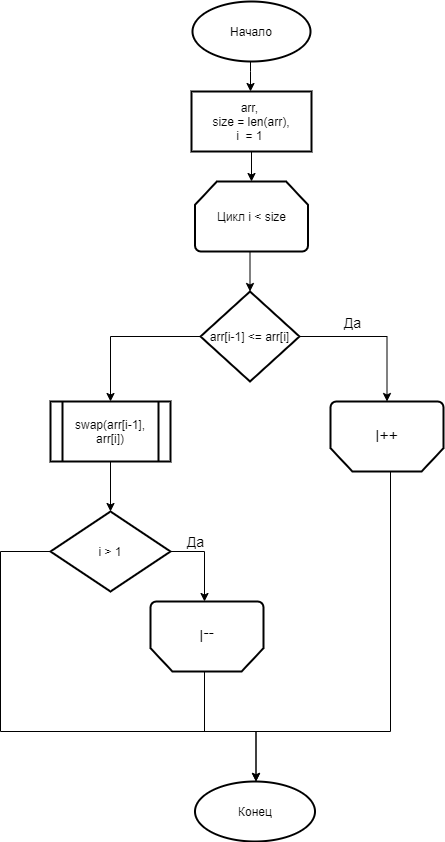
\includegraphics[scale=2.2]{gnome_graph}
		\centering \caption{Схема алгоритма гномьей сортировки}
	\end{figure}
	\clearpage
	\newpage
	\subsection{Трудоемкость алгоритмов}
	Введем модель трудоемкости для оценки алгоритмов:
	\begin{enumerate}
		\item базовые операции стоимостью 1 - +, -, *, /, =, ==, <=, >=, !=, +=, [], получение полей класса;
		\item оценка трудоемкости цикла: Fц = init + N * (a + Fтела + post) + a, \\где а - условие цикла, init - предусловие цикла, post - постусловие цикла;
		\item стоимость условного перехода применим за 0, стоимомть вычисления условия остаётся. 
	\end{enumerate}
	Далее будет приведены оценки трудоемкости алгоритмов.
	\subsubsection{Сортировка пузырьком}
	\hspace*{5mm} {\bf Лучший случай: } Массив отсортирован; не произошло ни одного обмена за 1 проход -> выходим из цикла.
	\\ Трудоемкость: 1 + 1 + 2 + {\it n} * (2 + 7 + 1 + 3) = 13n + 4 = {\it O(n)}.
	\\ \hspace*{5mm} {\bf Худший случай: } Массив отсортирован в обратном порядке; в каждом случае происходил обмен.
	\\ Трудоемкость: 1 + 1 + 2 + {\it n} * ({\it n} * (7 + 5 + 1 + 3) + 1 + 1) = 16$n^2$ + 2n + 4 = {\it O($n^2$)}.
	
	\subsubsection{Сортировка вставками}
	\hspace*{5mm} {\bf Лучший случай: } Массив отсортирован. При этом все внутренние циклы состоят всего из одной итерации.
	\\ Трудоемкость: T(n) = 3n + ((2 + 2 + 4 + 2) * (n - 1)) = 3n + 10(n - 1) = 13n - 10 = {\it O(n)}.
	\\ \hspace*{5mm} {\bf Худший случай: } Массив отсортирован в обратном порядке; каждый новый элемент сравнивается со всеми в отсортированной последовательности. Все внутренние циклы будут состоять из j итераций.
	\\ Трудоемкость:  T(n) = 3n + (2 + 2)(n - 1) + 4($\frac{n(n+1)}{2}$) - 1) + 5$\frac{n(n-1)}{2}$ + 3(n-1) = 3n + 4n - 4 + 2$n^2$ + 2n - 4 + 2.5$n^2$ - 2.5n + 3n - 3 = 4.5$n^2$ + 9.5n - 11 = {\it O($n^2$)}.

	\clearpage
	\newpage
	\subsubsection{Гномья сортировка}
	\hspace*{5mm} {\bf Лучший случай: } Массив отсортирован; не произошло ни одного обмена.
	\\ Трудоемкость: 1 + 1 + 1 + {\it n} * (1 + 4 + 1) = 6n + 3 = {\it O(n)}.
	\\ \hspace*{5mm} {\bf Худший случай: } Массив отсортирован в обратном порядке; в каждом случае происходил обмен.
	\\ Трудоемкость: 1 + 1 + 1 + {\it n} * (2 + {\it n} * (3 + 1 + 1)) = 5$n^2$ + 2n + 3 = {\it O($n^2$)}.
	
	\subsection{Вывод}
	\hspace*{5mm} В данном разделе были рассмотрены схемы алгоритмов сортировки массива. Введена модель оценки трудоемкости алгоритма, были расчитаны трудоемкости алгоритмов в соответствии с этой моделью. \newline
	\\ Сортировка пузырьком: лучший - {\it O(n)}, худший - {\it O($n^2$)}.
	\\ Сортировка вставками: лучший - {\it O(n)}, худший - {\it O($n^2$)}.
	\\ Гномья сортировка: лучший - {\it O(n)}, худший - {\it O($n^2$)}. \newline
	\\ \hspace*{5mm} При этом сортировка вставками быстрее пузырька в худшем случае т.к. имеет меньший коэффициент. Вставки 4.5$n^2$, пузырек 16$n^2$	
\end{flushleft}

\newpage
\section{Технологическая часть}
\begin{flushleft}
	\hspace*{5mm} В данном разделе будут рассмотрены требования к программному обеспечению, средства реализации и представлен листинг кода.
	\subsection{Требования к программному обеспечению}
	\hspace*{5mm} Входные данные: массив.
	\\ \hspace*{5mm} Выходные данные: отсортированный массив.
	\\ \hspace*{5mm} На рисунке 4 представлена IDEF0-диаграмма, показывающая функциональную схему сортировки массива.
	\begin{figure}[h]
		
		\centering 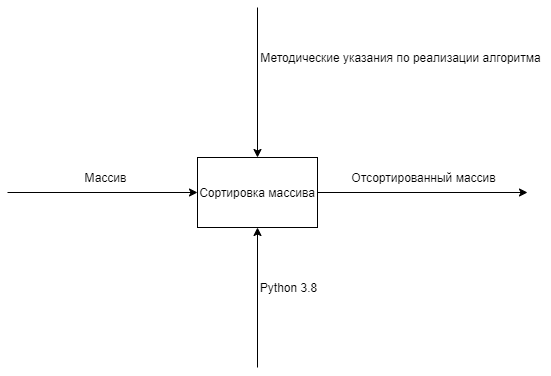
\includegraphics[scale=0.8]{диаграмма}
		\centering\caption{IDEF0-диаграмма, описывающая функциональную схему сортировки массива.}
	\end{figure}
	\subsection{Средства реализации}
	\hspace*{5mm} В данной работе используется язык программирования Python, так как ЯП позволяет написать программу за кратчайшее время. Проект выполнен в среде разработки Visual Studio Code.
	\clearpage
	\newpage
	\subsection{Листинг кода}
	В данном пункте представлен листинг кода алгоритмов сортировик.\cite{yandexSortAlg} А именно:
	\begin{itemize}
		\item алгоритм сортировки пузырьком;
		\item алгоритм сортировки вставками;
		\item алгоритм гномьей сортировки.
	\end{itemize}
	\definecolor{codegreen}{rgb}{0,0.6,0}
	\definecolor{codegray}{rgb}{0.5,0.5,0.5}
	\definecolor{codepurple}{rgb}{0.58,0,0.82}
	\definecolor{backcolour}{rgb}{0.95,0.95,0.92}

	\lstdefinestyle{mystyle}{
		backgroundcolor=\color{backcolour},   
		commentstyle=\color{codegreen},
		keywordstyle=\color{magenta},
		numberstyle=\tiny\color{codegray},
		stringstyle=\color{codepurple},
		basicstyle=\ttfamily\footnotesize,
		breakatwhitespace=false,         
		breaklines=false,                 
		captionpos=b,                    
		keepspaces=true,                 
		numbers=left,                    
		numbersep=5pt,                  
		showspaces=false,                
		showstringspaces=false,
		showtabs=false,                  
		tabsize=4
	}

	\lstset{style=mystyle}

	\hspace*{5mm} На листинге 1 представлен код алгоритма сортировки массива пузырьком.
	\begin{lstlisting}[language=Python, caption = Алгоритм сортировки пузырьком]
		def bubbleSort(arr):
			size = len(arr) 
			for i in range(size):
				for j in range(0, size-i-1):
					if arr[j] > arr[j+1]:
						arr[j], arr[j+1] = arr[j+1], arr[j]
			return arr
	\end{lstlisting}

	\hspace*{5mm} На листинге 2 представлен код алгоритма сортировки массива вставками.
	\begin{lstlisting}[language=Python, caption = Алгоритм сортировки вставками]
		def insertSort(arr):
			size = len(arr)
			for i in range(size):
				j = i - 1
				key = arr[i]
				while arr[j] > key and j >= 0:
					arr[j+1] = arr[j]
					j -= 1
				arr[j+1] = key
			return arr
	\end{lstlisting}
	\clearpage
	\newpage
	\hspace*{5mm} На листинге 3 представлен код алгоритма сортировки массива гномьей сортировкой.
	\begin{lstlisting}[language=Python, caption =  Алгоритм гномьей сортировки]
		def gnomeSort(arr):
			i, size = 1, len(arr)
			while i < size:
				if arr[i - 1] <= arr[i]:
					i += 1
				else:
					arr[i - 1], arr[i] = arr[i], arr[i - 1] 
					if i > 1:
						i -= 1
			return arr
	\end{lstlisting}
	\subsection{Вывод}
	\hspace*{5mm} В данном разделе была представлена структура ПО и листинги кода программы. 
	
\end{flushleft}

\newpage
\section{Исследовательская часть }
\begin{flushleft}
	\hspace*{5mm} В данном разделе будет проведен эксперимент и сравнительный анализ.
	\subsection{Системные характеристики}
	Характеристики компьютера на котором проводился замер времени сортировки массива:
	\begin{enumerate}
		\item операционная система - Windows 10;
		\item процессор - Intel(R) Core(TM) i7-10510U CPU @1.80GHz 2.30GHz;
		\item оперативная память - 16 ГБ.
	\end{enumerate}
	\subsection{Постановка эксперимента}
	В рамках данного проекта были проведены эксперименты, описанные ниже:
	\begin{enumerate}
		\item сравнение времени работы алгоритмов сортировки при разных заполнениях.
	\end{enumerate}
	\subsection{Сравнительный анализ на основе замеров времени работы алгоритмов}
	Был проведен замер времени работы каждого из алгоритмов.
	\clearpage
	\newpage
	\hspace*{5mm} На рисунке 5 представлен первый эксперимент, где он производится для лучшего случая, когда массив уже отсортирован.
	\begin{figure}[h]
		\centering 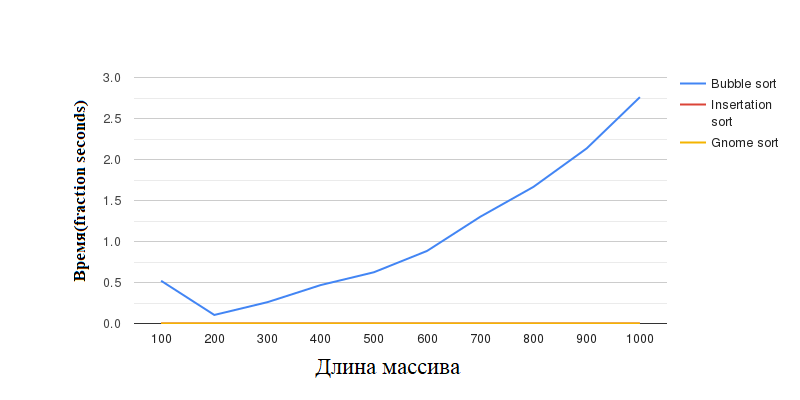
\includegraphics[scale=2.1]{sorted}
		\centering\caption{Сравнение времени работы алгоритмов сортировки, в уже отсортированном массиве}
	\end{figure}
	\clearpage
	\newpage
	\hspace*{5mm} На рисунке 6 представлен второй эксперимент, где он производится для худшего случая, когда массив отсортирован в обратном порядке. Ниже приведена полученная диаграмма: 
	\begin{figure}[h]
		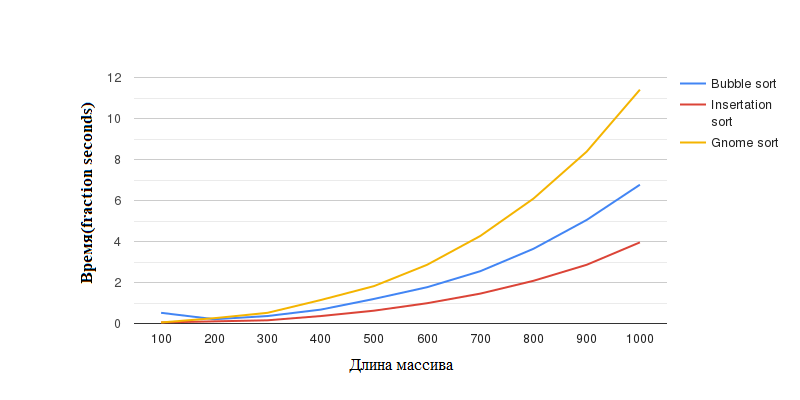
\includegraphics[scale=2.1]{reversed}
		\centering\caption{Сравнение времени работы алгоритмов в обратно отсортированном массиве}
	\end{figure}

	\clearpage
	\newpage
	\hspace*{5mm} На рисунке 7 производится третий эксперимент для общего случая, когда массив заполнен рандомными значениями. Ниже приведена полученная диаграмма: 
	\begin{figure}[h]
		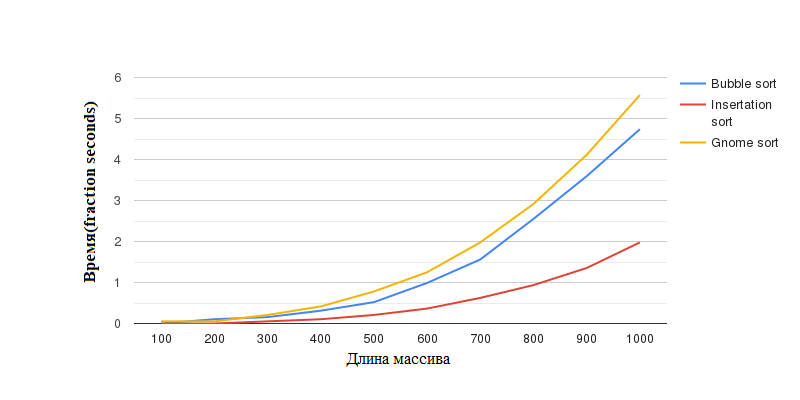
\includegraphics[scale=2]{random}
		\centering\caption{Сравнение времени работы алгоритмов при случайн заполнении массива}
	\end{figure}


	\subsection{Тестирование программы}
	В данном разделе будут показаны результаты тестирования
	\\ \hspace*{5mm} Всего было реализовано 5 тестовых случаев:
	\begin{enumerate}
		\item отрицательный размер массива;
		\item размер матрицы равен = 0;
		\item сравнение работы все трех алгоритмов на уже отсортированных значениях массива;
		\item сравнение работы все трех алгоритмов на обратно отсортированных значениях массива;
		\item сравнение работы все трех алгоритмов на случайных значениях массива;
	\end{enumerate}
	\clearpage
	\newpage
	\hspace*{5mm} На рисунке 8 предоставлен результат программы при вводе отрицательного значения для размера массива.
	\begin{figure}[h]
		\centering 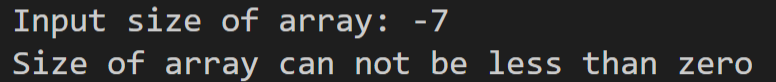
\includegraphics[scale=1.2]{zero}
		\centering\caption{Результат программы при отрицательном размере массива}
	\end{figure}
	\\ \hspace*{5mm} На рисунке 9 предоставлен результат программы при вводе размера массива равного нулю.
	\begin{figure}[h]
		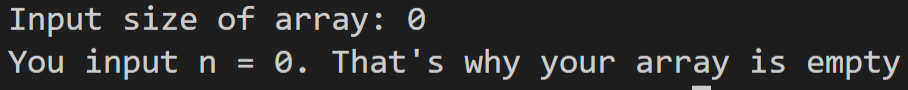
\includegraphics[scale=1.2]{less}
		\centering\caption{Результат программы при нулевом размере массива}
	\end{figure}
	\\ \hspace*{5mm} На рисунке 10 предоставлен результат программы при уже отсортированных значениях массива.
	\begin{figure}[h]
		\centering 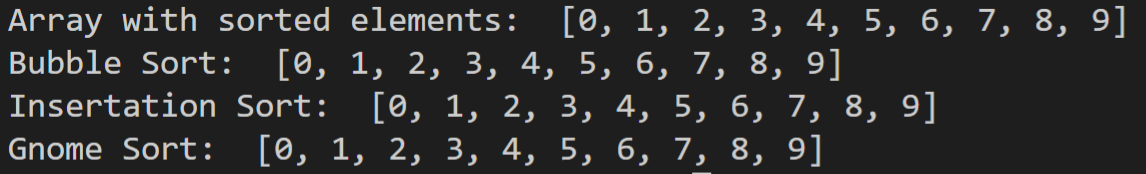
\includegraphics[scale=1.2]{sorted_test}
		\centering\caption{Результат программы при уже отсортированных значениях массива}
	\end{figure}
	\\ \hspace*{5mm} На рисунке 11 предоставлен результат программы при обратно отсортированных значениях массива.
	\begin{figure}[h!]
		\centering 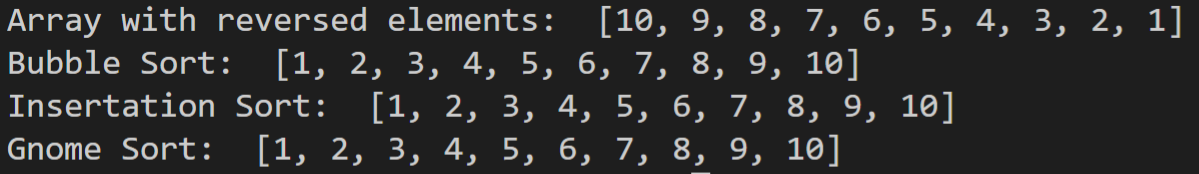
\includegraphics[scale=1.2]{reversed_test}
		\centering\caption{Результат программы при обратно отсортированных значениях массива}
	\end{figure}
	\clearpage
	\newpage
	\hspace*{5mm} На рисунке 12 предоставлен результат программы при случайных значениях массива.
	\begin{figure}[h!]
		\centering 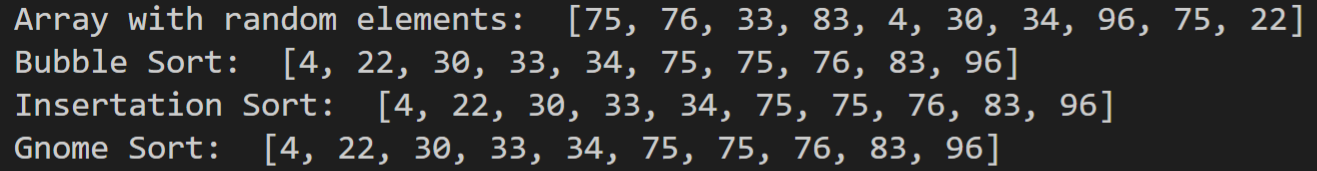
\includegraphics[scale=1.2]{random_test}
		\centering\caption{Результат программы при случайных значениях массива}
	\end{figure}
	\subsection{Вывод}
	\hspace*{5mm} По результатам тестирования все рассматриваемые алгоритмы сортировки были реализованы верно. Самым быстрым алгоритмом при случайном заполнении, оказался алгоритм сортировки вставками, а самым медленным - алгоритм гномьей сортировки. А алгоритм сортировки пузырьком, показал схожий результат с алгоритмом гномьей сортировки.
\end{flushleft}

\begin{flushleft}
	\newpage
	\section*{Заключение}
	\hspace*{5mm} В ходе работы были изучены алгоритмы сортировки массива: пузырьком, вставки, гномья. Выполнено сравнение всех рассматриваемых алгоритмов. Входе исследования был найден отпимальный алгоритм. Изучены зависимости выполнения алгоритмов от длины массива. Также был реализован программный код продукта.
	
\end{flushleft}

\clearpage
\newpage

\printbibliography



\end{document}